\section{Results}
\label{Results}
%
Of the 10 green categories we chose to exemplify four categories which are related to the robot’s appearance (udseende), behaviour (væremåde), approach (henvendelse), and trust (tillid). Based on these categories a variable can be elicitated according to the criterion of a) being an adjustable variable and b) the possibility of formulating the variables as a scale question. Because the field study is conducted with Danish speaking test subjects the variables are listed in both English and Danish. For each of the four main categories the following variables can be elicitated and formulated as a scale question:\\
%
\begin{itemize}
\item Appearance
\begin{enumerate}
  \item I think R's height is (Jeg synes at R's højde er)
  \item I think R is elegant (Jeg synes R er elegant)
  \item I think R looks human (Jeg synes R ser menneskelig ud)
  \item I like R's look (Jeg kan godt lide R's udseende)
\end{enumerate}
\item Behaviour
\begin{enumerate}
  \item I think R's movements are calm (Jeg synes R har rolige bevægelser)
  \item I think R's speed is (Jeg synes at R's hastighed er)
  \item I think R is annoying (Jeg synes R er irriterende)
  \item I think R is alive (Jeg synes R er levende)
  \item I think R is intrusive (Jeg synes R er anmassende)
\end{enumerate}
\item Approach 
\begin{enumerate}
  \item I think R is accommodating (Jeg synes R er imødekommende)
  \item I thought that R came too close to me (Jeg synes R kom for tæt på)
  \item I thought that R was blocking my way (Jeg synes R stod i vejen)
  \item I was surprised by R's approach (Jeg blev overrasket over R's henvendelse)
  \item I thought that R was intimidating (Jeg synes R er intimiderende)
\end{enumerate}
\item Trust 
\begin{enumerate}
  \item I feel safe around R (Jeg føler mig tryg ved R)
  \item I count on R to follow me to the right place (Jeg regner med at R følger mig hen til det sted jeg har valgt)
  \item R scared me (R gjorde mig forstrækket)\\
\end{enumerate}
\end{itemize}
%
In the above scale questions \textit{R} is short for robot. In the following tabels each individual scale question is listed alongside the labels on the specific scale. If the scale does not contain a mid point it will be noted with \textit{-}, if it contains an unlabeled mid point it will be noted with \textit{No label}, whereas if the mid point is label the specific label is noted. 
%
\begin{table}[H]
	\centering
	\begin{tabular}{l|c|c|c}
		Scale question     & Left label & Right label & Mid point \\\hline
		1   & Too low (for lav) & Too high (for høj) & Appropriate (fin)         \\\hline
		2   & Not at all elegant (slet ikke elegant) & Extremely elegant (ekstremt elegant) & -         \\\hline
		3   & Not at all human (slet ikke menneskelig) & Extremely human (ekstremt menneskelig) & -         \\\hline
	 	4   & (kan slet ikke lide R's udseende) & (kan ekstremt godt lide R's udseende) & -         \\\hline
		5   & Not at all scared (slet ikke forskrækket) & Extremely scared (ekstremt forskrækket) & -           
	\end{tabular}
	\caption{Specific scale labels for each scale question concerning the robots appearance.}
	\label{tab:Latin}         
\end{table}
\noindent
%

%
\begin{table}[H]
	\centering
	\begin{tabular}{l|c|c|c}
		Scale question     & Left label & Right label & Mid point \\\hline
		1   & Very calm (meget rolige) & Very wild (meget vilde) & No label          \\\hline
		2   & Too slow (for langsom) & Too fast (for hurtig) & Appropriate (fin)         \\\hline
		3   & Not at all annoying (slet ikke irriterende) & Extremely annoying (ekstremt irriterende) & -         \\\hline
	 	4   & Not at all alive (slet ikke levende) & Extremely alive (ekstremt levende) & -         \\\hline
		5   & Not at all intrusive (slet ikke anmassende) & Extremely intrusive (ekstremt anmassende) & -            
	\end{tabular}
	\caption{Specific scale labels for each scale question concerning the robots behavior.}
	\label{tab:Latin}         
\end{table}
\noindent
%

%
\begin{table}[H]
	\centering
	\begin{tabular}{l|c|c|c}
		Scale question     & Left label & Right label & Mid point \\\hline
		1   & Very rejective (meget afvisende) & Very accommodating (meget imødekommende) & No label          \\\hline
		2   & Too far (for langt væk) & Too close (for tæt på) & Appropriate (tilpas)         \\\hline
		3   & Not at all blocking my way (slet ikke i vejen) & Extremely blocking my way (ekstremt i vejen) & -         \\\hline
	 	4   Not at all surprised (slet ikke overrasket) & Extremely surprised (ekstremt overrasket) & -         \\\hline
		5   & Not at all intimidating (slet ikke intimiderende) & Extremely intimidating (ekstremt intimiderende) & -           
	\end{tabular}
	\caption{Specific scale labels for each scale question concerning the robots approach.}
	\label{tab:Latin}         
\end{table}
\noindent
%

%
\begin{table}[H]
	\centering
	\begin{tabular}{l|c|c|c}
		Scale question     & Left label & Right label & Mid point \\\hline
		1   & \makecell{Extremely unsafe\\ (ekstremt utryg)} & Extremely safe (ekstremt tryg) & No label          \\\hline
		2   & Completely disagree (helt uenig) & Completely agree (helt enig) & Neutral 
	\end{tabular}
	\caption{Specific scale labels for each scale question concerning the users trust in regard of the robot.}
	\label{tab:Latin}         
\end{table}
\noindent
%
The scale questions can either be presented on a bi- or unipolar \textit{Visual Analoge Scale} (VAS) with open anchor points. If the scale is bipolar a midt point will be marked. In writing, the scales have not been properly developed but are expected to appear as shown on \autoref{fig:Height} and \autoref{fig:HumanMenneskelig} bipolar and unipolar respectively.
%
\begin{figure}[H]
\centering

\includegraphics[width = 0.49\textwidth]{Figure/HeightHoejde} 
\caption{Example of a bipolar scale relevant for the scale question: \textit{I think R's height is}.}
\label{fig:Height}
\end{figure}
\noindent
% 
An example of an unipolar scale is illustrated on \autoref{fig:HumanMenneskelig}.
%
\begin{figure}[H]
\centering
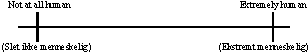
\includegraphics[width = 0.49\textwidth]{Figure/HumanMenneskelig} 
\caption{Example of an unipolar scale relevant for the scale question: \textit{I think R looks human}.}
\label{fig:HumanMenneskelig}
\end{figure}
\noindent
%
